\documentclass[]{standalone}

\usepackage{adjustbox}

\usepackage{amsmath}

\usepackage{mathrsfs}

\usepackage{tikz}
\usetikzlibrary{arrows, patterns, decorations.pathmorphing, backgrounds, positioning, fit, petri, shapes, trees, matrix, chains, decorations, decorations.pathreplacing, decorations.fractals, calc,snakes,trees, decorations.markings}

\usepackage{color}
\definecolor{soton}{RGB}{7,51,71}
\colorlet{comms}{red!50!yellow}
\colorlet{payld}{pink!50!purple}
\colorlet{obdh}{green!50!black}

\begin{document}

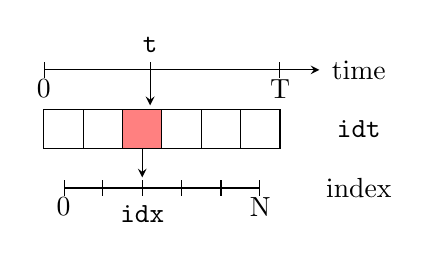
\begin{tikzpicture}
\draw[|-|] (0,0) node[below] {0} -- (3,0) node[below] {T};
\draw (1.35,-0.1) -- (1.35,0.1) node[above] {\verb!t!};
\node[above] (t) at (1.35,-0.1) {};
\draw[-stealth] (3,0) -- (3.5,0);
\node at (4,0) {time} ;

\begin{scope}[yshift=-1cm]
    \draw (0,0.5) rectangle (3,0);
    \foreach \x in {0.5,1,1.5,2,2.5}{
        \draw (\x, 0) -- (\x, 0.5);
        }
    \draw[fill=red!50] (1,0) rectangle (1.5,0.5);
    \node at (4,0.25) {\verb!idt!};
    \node[below] (idt) at (1.35,0.55) {};
    \node[above] (idtl) at (1.25,0) {};
\end{scope}

\begin{scope}[yshift=-1.5cm]
    \draw[|-|] (0.25,0) -- (2.75,0);
    \foreach \x in {0.75,1.25,1.75,2.25}{
        \draw (\x, -0.1) -- (\x, 0.1);
        }
    \node[below] at (0.25,0) {0};
    \node[below] at (2.75,0) {N};
    \node at (4,0) {index};
    \node (idx) at (1.25,0.01) {};
    \node[below] at (1.25,-0.1) {\verb!idx!};
\end{scope}

\draw[-stealth] (t) -- (idt);
\draw[-stealth] (idtl) -- (idx);

\end{tikzpicture}


\end{document}